\section{Introduction}
% neural networks paper für kurs
This paper is the result of fulfilling assignment 3 of the neural networks course in the university of Leiden.
It asks the students to portray a freely chosen research topic within the field of neural networks.
We chose to bring the topic of \textit{deep dreaming} closer to the reader.

% was machen wir eigentlich
Deep Dreaming enables the visualization of known features of a trained neural network.
Section \ref{sec:problemstatement} will inform why this was invented and how it is useful.
Section \ref{sec:previouswork} will then look at what similar things were done before the idea of \textit{deep dreaming}.
We then will go deep into the inner workings of the algorithm itself in Section \ref{sec:how} to explain why the visualization works.
We will use hand picked images and models, detailed in Section \ref{sec:data} to apply deep dreaming to. The results of these experiments will be displayed in Section \ref{sec:evaluation}, and possible conclusions drawn in Section \ref{sec:conclusion}.

% https://research.googleblog.com/2015/06/inceptionism-going-deeper-into-neural.html

\subsection{Problem Statement \& Motivation}
\label{sec:problem-statement}
% Warum machen wir das überhaupt?
Neural Networks with meaningful applications are complex structures with many layers, nodes and trained weights.
For example VGG19, an Image Categorisation Neural Network, consists of 19 Layers summing up to a total of 143,667,240 trained parameters\cite{vgg}. These weights were trained to recognize images and map them to a description string based on the ImageNet Dataset.
The problem one faces now is that there is no saying in what the individual layers and nodes have actually learned to respond to, or how the Neural Network actually draws a conclusion\cite{castelvecchi2016can}.
%  -> NN sind Blackboxes, haben zwar definierte Struktur, aber Zusammenspiel der Weights unbekannt
Such behaviour is often referred to as a \textit{black box} and one of the fundamental architectural problems in mastering neural networks\cite{olden2002illuminating}.

% besser nachvollziehen von klassifizierung durch besseres verständnis / visualisierung der gelernten merkmale
In order to get at least a small grasp of what these layers or nodes have learnt, an approach to visualize said knowledge is needed.
As maybe already apparent from the mention of VGG19, we are focusing on neural networks that process images.
Hence the visualization methods that will be portrayed in the coming chapters are limited to image processing neural networks and not generally applicable to \textit{decipher} any neural networks weights.

\subsubsection{Visualizing Learned Features}
% https://blog.keras.io/how-convolutional-neural-networks-see-the-world.html
In this chapter we will describe the visual aspect of the so called \textit{Deep Dream} visualization method.
A detailed mathematical explanation of how and why this works is given in Section \ref{sec:how}.
Deep Dreaming requires a pretrained image recognition neural network, and a source image one wishes to modify. The source image can be any arbitrary image.
Figure \ref{fig:neuronreact} portrays a small section of an abstract unspecified neural network.
The small image parts contained within each neurons are examples of features a neuron can learn to respond to. In this instance the feature was then applied to a random noise image.
One can pick out individual or a set of neurons,
and activate them on the source image to modify it in a way that the learnt features are embedded into it.
An example of this can be seen in Figure \ref{fig:applieddream}.
Here the neuron on the very top left of Figure \ref{fig:neuronreact} was chosen to be activated the most in order to modify the source image and the learnt feature now dominates the visual appearance of the image.
Since it would be close to impossible to find the right combination of neurons to draw a specific object, there is the possibility of a \textit{Guided Dream}.
The concrete inner workings of the \textit{Guided Dream} are explained in Section \ref{guided-dreaming}.
For a guided dream there is a second image in play, which we will refer to as \textit{Guide Image}.
This image is processed by the network and the neurons that responded the most to the features contained within it will then be used for the modification.
That way one could use a blank source image and a guide image, e.g. of a cat. By then selecting the strongest activated neurons by the guide we get an idea of which features the neural network learnt about cats.
An example of this can be seen in Figure \ref{fig:guided}.

\begin{figure}[H]
	\centering
	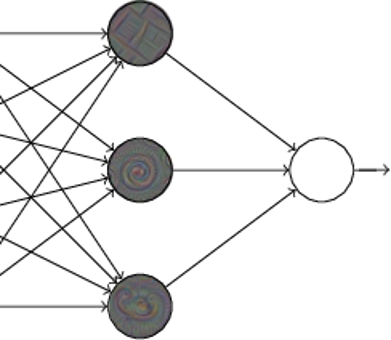
\includegraphics[width=0.5\linewidth]{img/neurons-reaction.png}
	\caption{A small section of an abstract unspecified neural network. Within the layers is the applied \textit{Deep Dream} visualizing the feature learnt by the neuron\cite{nielsen2015neural}.}
	\label{fig:neuronreact}
\end{figure}

\begin{figure}[H]
	\centering
	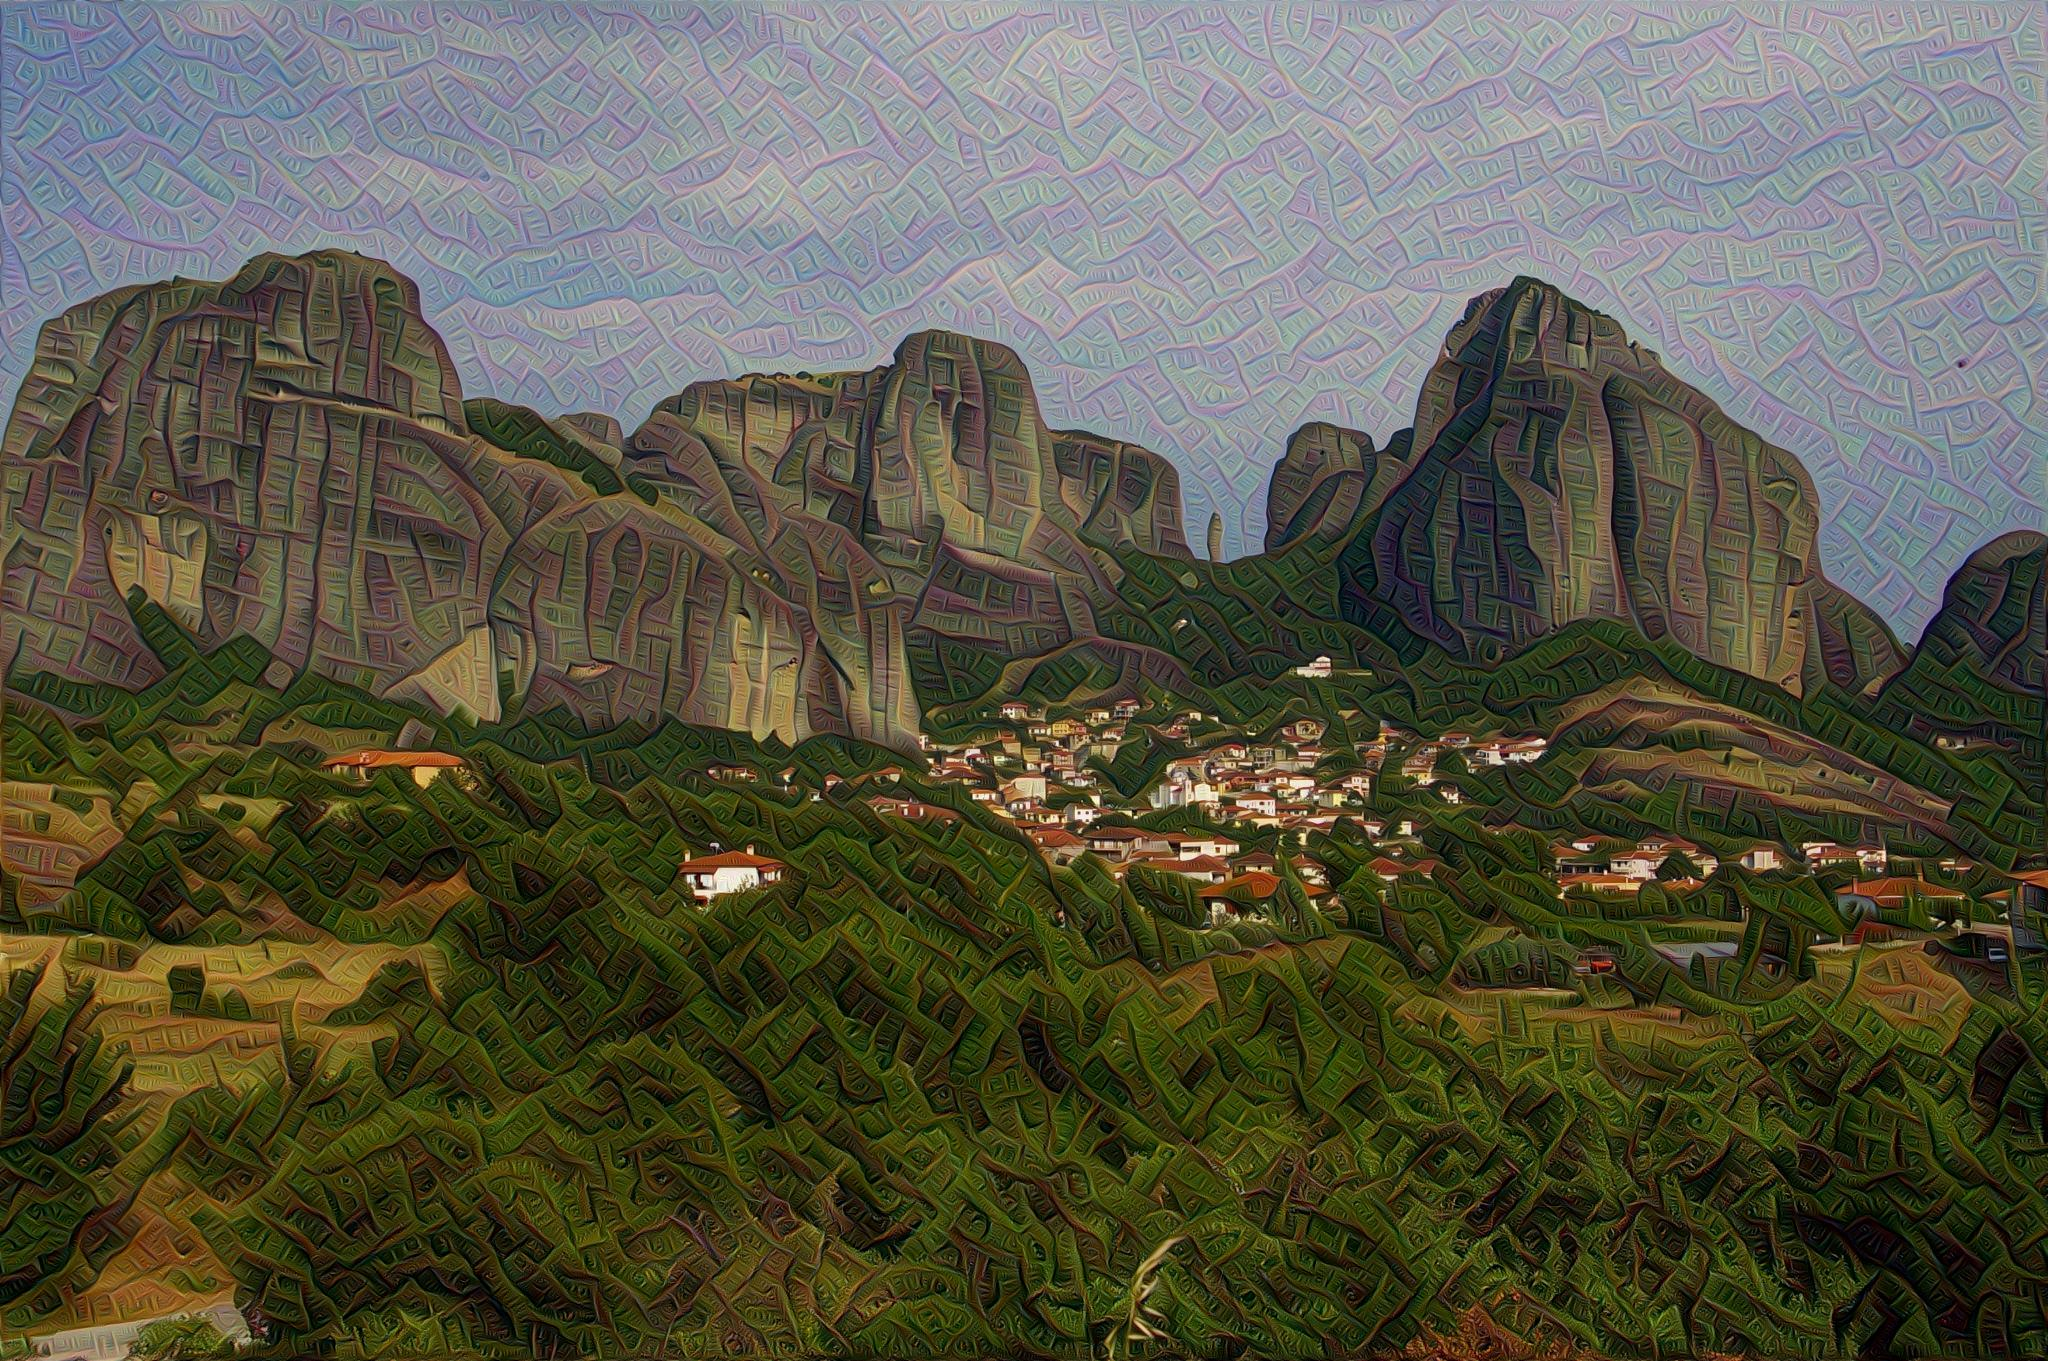
\includegraphics[width=0.5\linewidth]{img/applied_neuron.png}
	\caption{A \textit{Deep Dream} onto a Landscape image as source which maximizes one specific neuron reacting apparently to certain edge types.}
	\label{fig:applieddream}
\end{figure}

% https://research.googleblog.com/2015/06/inceptionism-going-deeper-into-neural.html

% weitere anwendungsbereiche
% interesting results
% fake features for misclassification